\documentclass{article}
\usepackage{amsmath}
\usepackage{amssymb}
\usepackage{graphicx}
\usepackage{hyperref}
\usepackage[version=4]{mhchem}

\title{Problem 3}
\date{}

\begin{document}
\maketitle

\section*{Problem}
\(A B C D\) is a convex quadrilateral. \(E\) and \(F\) are midpoints of diagonals \(B D, A C\), respectively. Show that \(E F>\frac{1}{2}(A B-C D)\)\\
\centering
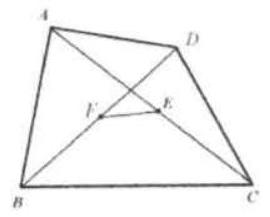
\includegraphics[width=\textwidth]{images/problem_image_1.jpg}

\section*{Solution}
Take \(N\), the midpoint \(B C\).\\
Connect the midpoints of \(E N\), and \(F N\), respectively. By Theorem 2.1, in triangle \(B D C, F N / / D C\), and

\[
F N=\frac{1}{2} D C
\]

By Theorem 2.1, in triangle \(C A B, E N / / A B\), and\\
\centering
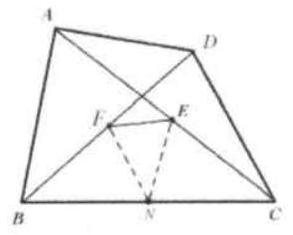
\includegraphics[width=\textwidth]{images/reasoning_image_1.jpg}

\[
E N=\frac{1}{2} A B
\]

(2) - (1): \(E N-F N=\frac{1}{2}(A B-C D)\)

By the triangle inequality theorem, \(E N-F N<E F\).\\
(3) can be written as \(E N-F N=\frac{1}{2}(A B-C D)<E N\), or \(E F>\frac{1}{2}(A B-C D)\).

\end{document}
